\leavevmode\newline \leavevmode\newline
{\centering
\noindent{\Large \textbf{Towards Linguistically and Culturally Inclusive LLMs}}\\  \vspace*{-0.1cm} \leavevmode\newline
{\normalsize \textbf{Partha Talukdar}}\\
{\normalsize {Google DeepMind, India}}\\


\begin{figure}[h!]
  \centering
      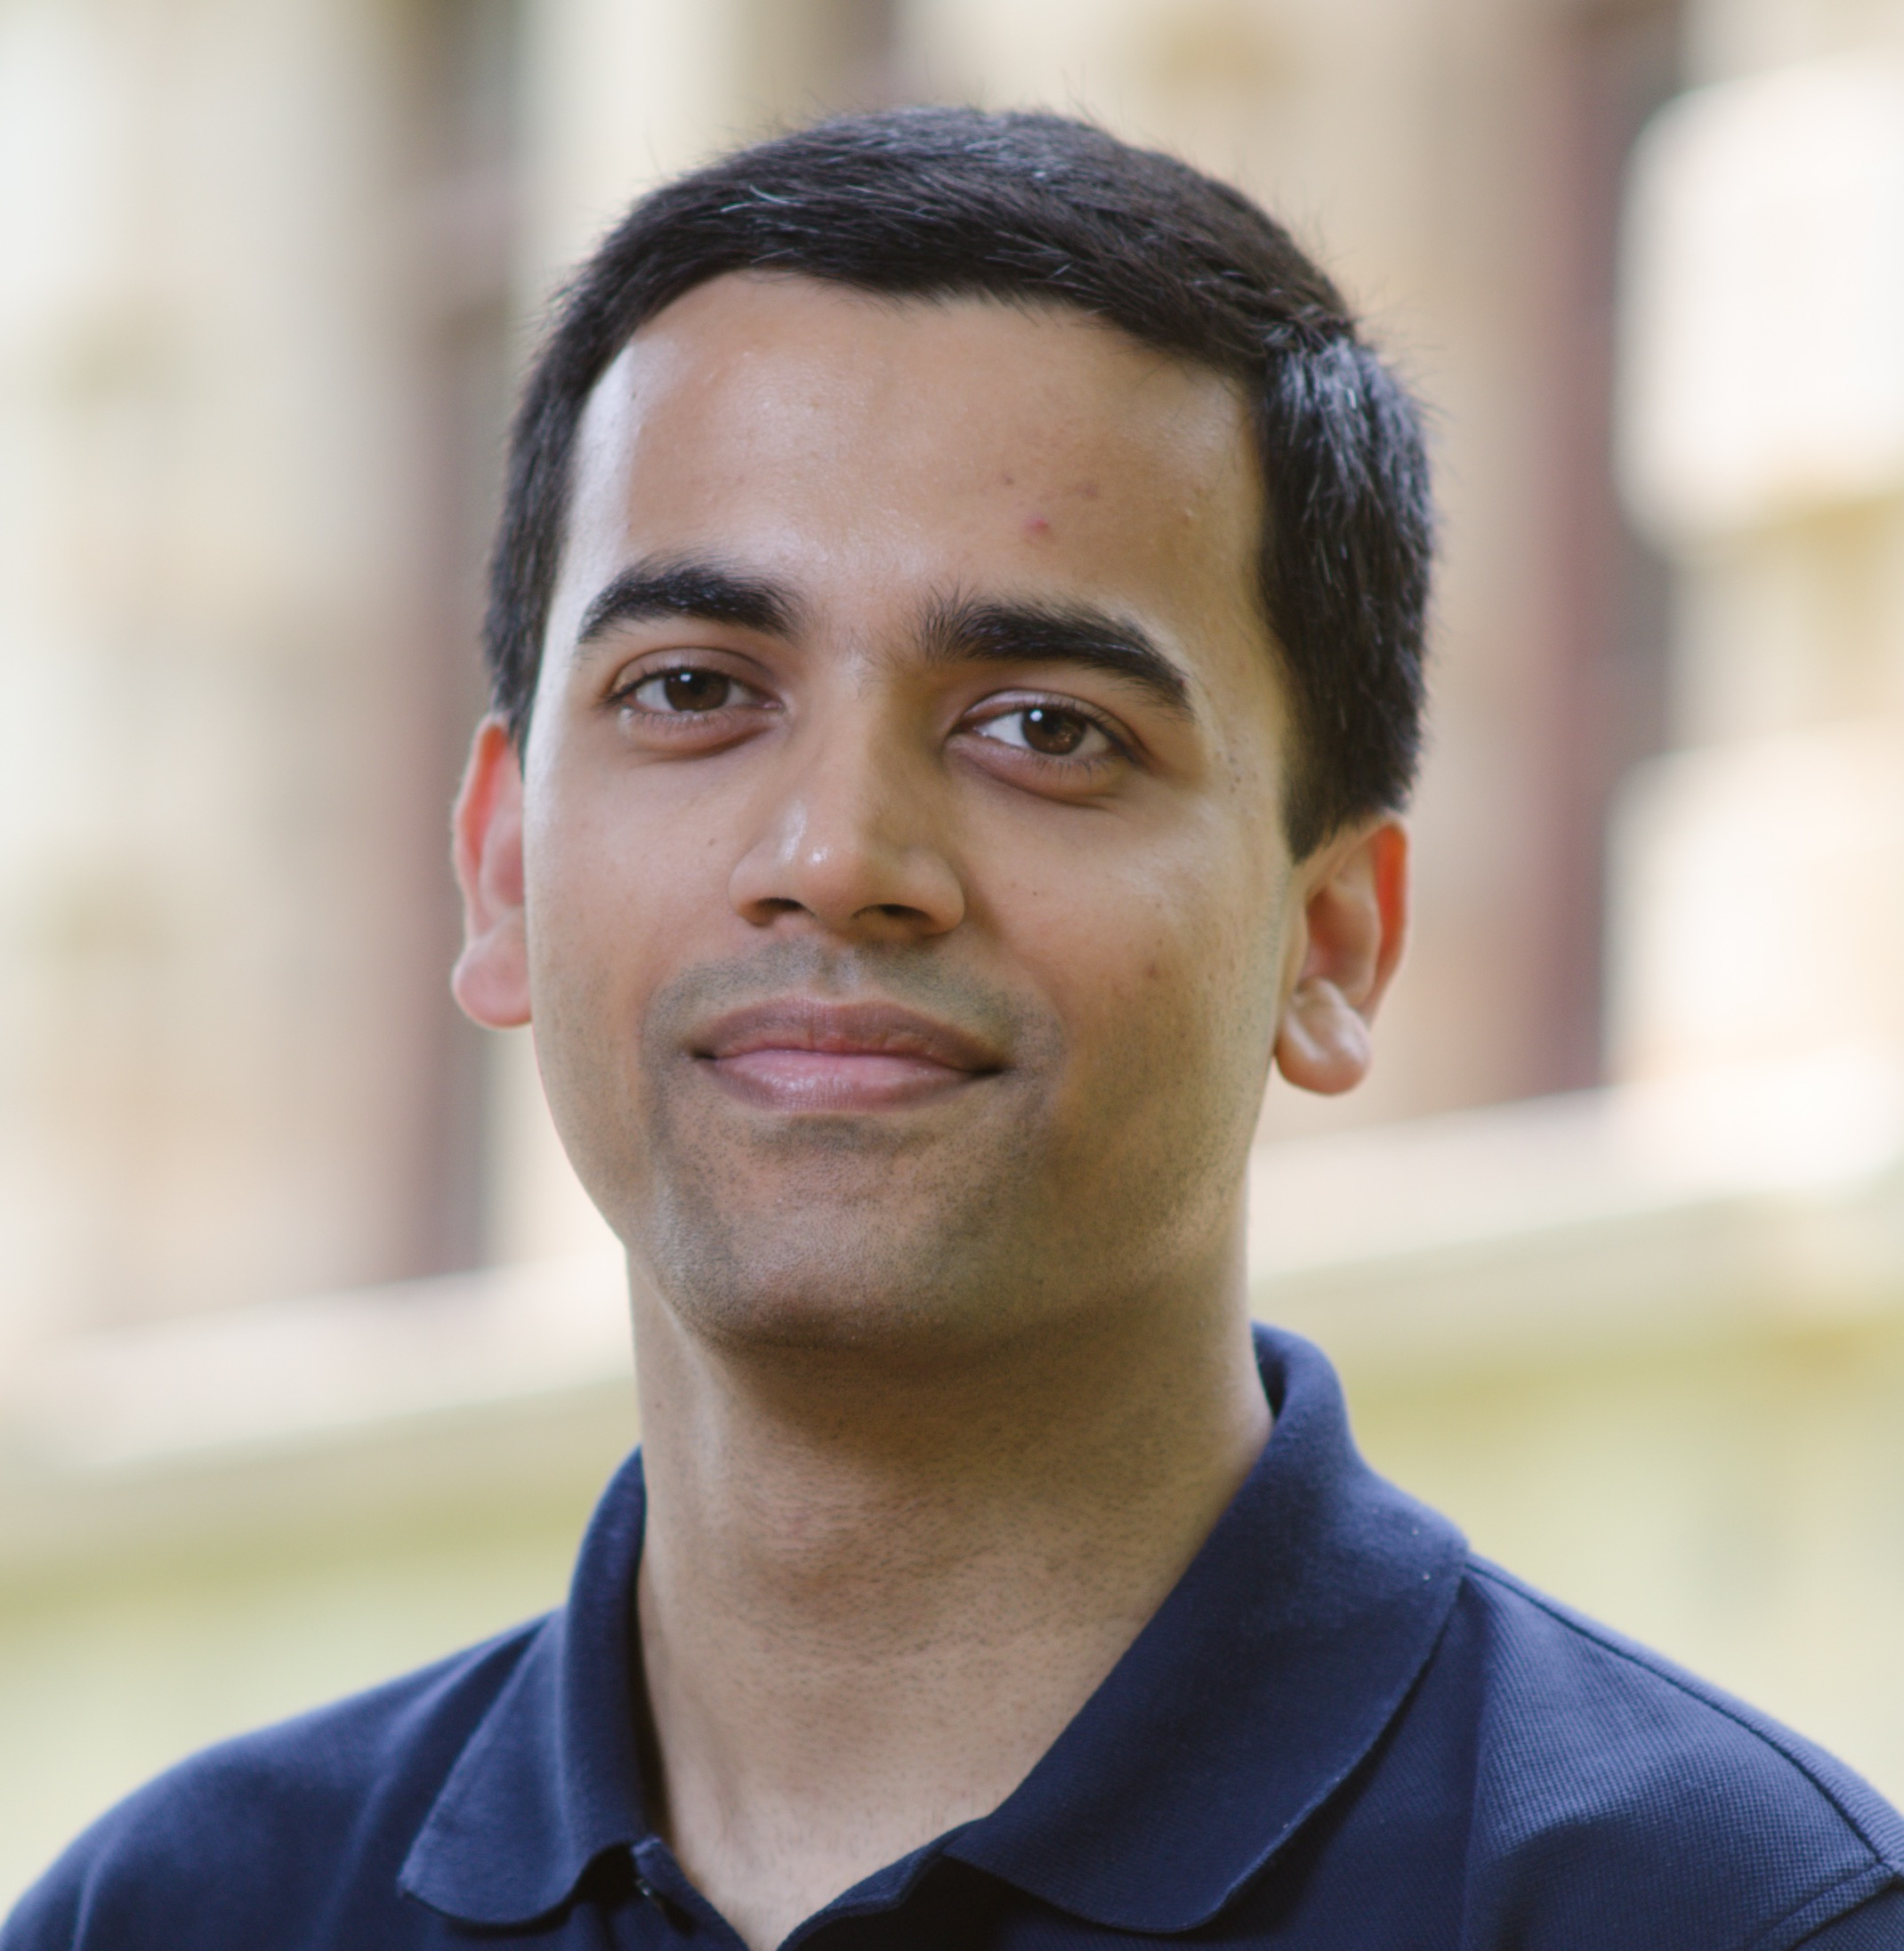
\includegraphics[width=0.15\linewidth]{examples/handbook_coling25/invited_talks/partha_invited_3.png}
\end{figure}

 {\normalsize \textbf{Friday, Jan 24, 2025} -
 Room: \textbf{???} -
 Time: \textbf{09:00-10:00}\\\leavevmode\newline
 }
}

{\textbf{Abstract:}}
Large Language Models (LLMs) have seen tremendous progress over the last few years with increasing adoption across the globe. Even though there are more than 7000 languages in the world, LLMs are currently usable in only a handful of them. Moreover, as LLMs get used across geographies, there is a need for them to become adaptive to regional cultural nuances and local norms. These raise interesting research challenges in language and culture, especially due to the limited availability of representative data and evaluations. In this talk, I shall present an overview of our research in this promising area of inclusive LLMs. I shall talk about Project Vaani where the goal is to capture and make available the speech landscape of India using a unique geo-anchored approach, modular approaches such as CALM to increase the scope of LLMs using composition, and benchmarks such as CUBE to evaluate the cultural knowledge of LLMs.\\

{\textbf{Bio:}}
Partha is a Researcher at Google DeepMind India where he leads the Languages group. He is also a Faculty Member at IISc Bangalore. Previously, Partha was a Postdoctoral Fellow in the Machine Learning Department at Carnegie Mellon University. He received his PhD (2010) from the University of Pennsylvania. Partha is broadly interested in making AI more inclusive with a view towards benefiting a broader part of the world population. Partha is a recipient of several awards, including an Outstanding Paper Award at ACL 2019 and the ACM India Early Career Award 2022. He is also a Fellow of the Indian National Academy of Engineering. He is a co-author of a book on Graph-based Semi-Supervised Learning. Homepage: https://parthatalukdar.github.io/\\

\clearpage